\section{Experiments}
\label{exp}
%introduction on how this chapter is structured

%Experimental Results (recommended size: 1.5 pages)
\subsection{Set-up}
%a. Experimental setup: describe the working environments (DAS, Amazon EC2,
%etc.), the general workload and monitoring tools and libraries, other tools and
%libraries you have used to implement and deploy your system, other tools and
%libraries used to conduct your experiments.
All of our experiment were run on Amazon EC2 t2.micro machines, these machines have only 1 CPU and 1GB of memory. We had rented 5 of them and had used them for all of our experiments. However, it is very easy to extend our application to support unlimited number of Virtual Machines. We were running the Amazon Linux operating system with a Java installation on all of our instances.

To perform the experiments, we have prepared 5 different ZIP files with different size containing different amount of images. The overview of this test set is in the table \ref{testset}.

\begin{table}
\centering
 \label{testset}
 \begin{tabular}{| l | c | c |}
  \hline
  Set name & ZIP size & Number of images \\
  \hline
  \hline
  1 & 1MB & 1\\
  2 & 5MB & 5\\
  3 & 10MB & 10\\
  4 & 50MB & 50\\
  5 & 100MB & 100\\
  \hline
 \end{tabular}

 \caption{Files used for experiments.}
\end{table}

\subsection{Experiment analysis}
%b. Experiments: describe the experiments you have conducted to analyze each
%system feature, then analyze them; use one sub-section per experiment. For
%each experiment, describe the workload, present the operation of the system,
%and analyze the results.

 %In the analysis, report:
%i. Charged-time = time that would have been charged using the
%Amazon EC2 timing approach (1-hour increments)
%ii. Charged-cost = cost that would have been charged using the
%Amazon EC2 charging approach, assuming 10 Euro-cents/charged hour
%iii. Service metrics of the experiment, such as runtime and response time of
%the service, etc.
%iv. (optional) Usage metrics of the experiment, such as per-VM and overall
%system usage and activity.

\subsubsection{Load balancing}
\label{load}
In this experiment we have simulated two scenarios, a flash crowd arrival of a number of clients with a random file out of Table \ref{testset} and a steady state scenario where clients connect every 1 to 5 seconds. 

The flash crowd experiment simulates 5, 10, 15 and 20 clients connecting simultaneously. The average runtime of a job for each scenario can be seen on Figure \ref{flash}. As the load ballancer does not have time to start new instances, we can see that the average run time scales almost linearly, as all of the jobs are scheduled to the same amount of slave Virtual machines. Charged time of this experiment would be 1 hour and charged cost 10 cents.

The steady state scenario connects a new client randomly after 1 to 5 seconds. We again tried to schedule 5, 10, 15 and 20 jobs. The average runtime of job for each scenario can be seen on Figure \ref{steady}. As the VM manager now has time to start new machines, jobs are allocated more equably. But as we use just 4 slave machines at maximum, there is still significant difference between 5 jobs and 10. However, the difference between 15 and 20 jobs is small. Charged time of this experiment would be 1 hour and charged cost 10 cents.

\begin{figure}
 \centering

 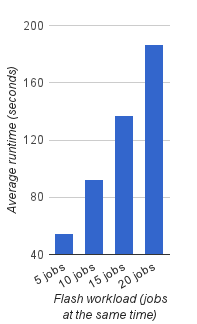
\includegraphics{flash-graph}
 \caption{Flash crowd arrival}
 \label{flash}
 \end{figure}

\begin{figure}
 \centering

 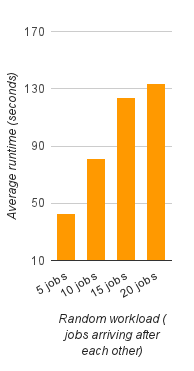
\includegraphics{random-graph}
 \caption{Steady state scenario}
  \label{steady}
\end{figure}

\subsubsection{Reliability}
When a machine fails, the client gets notified about this and has the possibility to resend the job. The system will recognize the failed machine and therefore it will start a new machine, which guarantees, that there will be a machine available to process the job. However, our reliability scenario does not count with the failure of the Master machine.

\subsubsection{Multi-Tenancy}
As seen in Section \ref{load}, multiple users can connect and run their job. By provisioning more machines, more users can be serviced. However more clients being processed on a machine means longer (but fair) processing time for all of the jobs, as could be seen on Figure \ref{flash}.